%\documentclass[a4paper,twoside,10pt]{article}
\interfootnotelinepenalty=10000
\usepackage[USenglish]{babel} %francais, polish, spanish, ...
\usepackage[T1]{fontenc}
%\usepackage[ansinew]{inputenc}
\usepackage{color}
\usepackage{mathtools}
%\usepackage{hyperref}
\usepackage{subfig}
\usepackage{multirow, booktabs}
\usepackage{hyperref}


\usepackage{lmodern} %Type1-font for non-english texts and characters
\usepackage{algorithm}
\usepackage[noend]{algpseudocode}
\usepackage{mnsymbol}

%% Packages for Graphics & Figures %%%%%%%%%%%%%%%%%%%%%%%%%%
\usepackage{graphicx} %%For loading graphic files
\usepackage{amsmath}
\usepackage{amsthm} 
\usepackage{thmtools}
\usepackage{amsfonts}
\usepackage[all,cmtip]{xy}
\usepackage{tikz}

\usepackage{TechFront}
%\declaretheorem{Lemma}
%\declaretheorem{prop}

\newcommand{\lre}{\color{red}{\{}}

%\DeclareMathOperator{\sign}{sgn}
%\DeclareMathOperator{\coef}{coef}
%\DeclareMathOperator{\var}{var}
%\DeclareMathOperator{\eqs}{eqs}
%\DeclareMathOperator{\feas}{feas}
%\DeclareMathOperator{\UB}{UB}
%\DeclareMathOperator{\lb}{lb}
%\DeclareMathOperator{\FMcomb}{FM-comb}
%\DeclareMathOperator{\Gcomb}{Gauss-comb}
%\DeclareMathOperator{\proj}{proj}
%\DeclareMathOperator{\Pos}{Pos}
%\DeclareMathOperator{\Neg}{Neg}
%\DeclareMathOperator{\rhs}{rhs}
\newcommand{\sign}{\mathit{sgn}}
\newcommand{\coef}{\mathit{co}}
\newcommand{\var}{\mathit{var}}
\newcommand{\VAR}{\mathit{VAR}}
\newcommand{\eqs}{\mathit{eqs}}
\newcommand{\feas}{\mathit{feas}}
\newcommand{\UB}{\mathit{UB}}
\newcommand{\UBc}{\mathit{UBineq}}
\newcommand{\lb}{\mathit{lb}}
\newcommand{\lbc}{\mathit{lbineq}}
\newcommand{\FMcomb}{\mathit{FM}}
\newcommand{\Gcomb}{\mathit{GA}}
\newcommand{\proj}{\mathit{proj}}
\newcommand{\Pos}{\mathit{Pos}}
\newcommand{\Neg}{\mathit{Neg}}
\newcommand{\rhs}{\mathit{rhs}}
\newcommand{\bounds}{\mathit{bounds}}
\newcommand{\ie}{\mathcal{IE}}
\newcommand{\xx}{\mathcal{X}}
\newcommand{\vea}{\mathbf{co}}
\newcommand{\ttt}{\texttt{t}}
\newcommand{\trt}[1]{\texttt{#1}}
\newcommand{\mi}{\mathit}

\newcommand{\false}{\texttt{false}}
\newcommand{\true}{\texttt{true}}
\newcommand{\nul}{\texttt{null}}
\newcommand{\ve}{\mathbf}
%\newcommand\lhs[1]{\text{lhs}(#1)}
%\newcommand\rhs[1]{\text{rhs}(#1)}
%\newcommand\coef[1]{\text{coef}(#1)}
%\newcommand\LB[1]{\text{LB}_{#1}}
%\newcommand\UB[1]{\text{UB}_{#1}}
\newcommand{\lig}[4]{\ve{#1}\cdot\ve{#2}#3#4}
\newcommand\red[1]{\textcolor{red}{#1}}
\newcommand\blue[1]{\textcolor{blue}{#1}}
\newcommand{\set}[2]{\{\;{#1}\;|\;{#2}\;\}}
\newcommand{\odef}{\overset{\text{def.}}=}
\newcommand{\mc}{\mathcal}
\algdef{SE}[DOWHILE]{Do}{doWhile}{\algorithmicdo}[1]{\algorithmicwhile\ #1}%
\newcommand{\argmin}{\operatornamewithlimits{argmin}}
\newcommand{\StateInd}{\State\hspace{\algorithmicindent}}
\newcommand{\pr}{\mathit{PR}}
\newcommand{\prs}{\mathit{PRS}}
\newcommand{\ens}{\Leftrightarrow}

%\algdef{SE}[DOPAR]{DoPar}{doParWhile}{\algorithmicdo\textbf{ in parallel for\ }}[1]{\algorithmicwhile\ #1}%
\algdef{SE}[DOPAR]{DoPar}{doParUntil}{\algorithmicdo\textbf{ in parallel for\ }}[1]{\algorithmicuntil\ #1}%

\algdef{SE}[SUBALG]{Indent}{EndIndent}{}{\algorithmicend\ }%
\algtext*{Indent}
\algtext*{EndIndent}

\newtheorem{prop}{Proposition}
\newtheorem{lemma}{Lemma}
\newtheorem{cor}{Corollary}

\newcounter{para}
%\newcommand\mypara[1]{\par\refstepcounter{para}\textbf{\thep‌​ara\space#1\space}}
\newcommand\mypara[1]{\newline\par\refstepcounter{para}\textbf{\thepara}\space \textbf{#1} \space}
%\newcommand\mypara{\par\refstepcounter{para}\thepara\space}
%\usepackage[thmmarks,...]{ntheorem}
\newcommand{\Sec}{F}
\newcommand{\Ca}{\mi{Cap}}
\newcommand{\Vol}{\mi{V}}
\newcommand{\Weight}{\mi{W}}
\newcommand{\weight}{\mi{w}}
\newcommand{\BonjeanStations}{\mi{BS}}
\newcommand{\bonjean}{bf}
\newcommand{\Bonj}{B}
\newcommand{\shear}{\mi{sf}}
\newcommand{\Prop}{P}

\theoremstyle{definition}
%\newtheorem{example}{Example}[section]
\newtheorem*{theorem}{Theorem}

\theoremstyle{definition}
\newtheorem{examplex}{Example}[section]
\newenvironment{example}
  {\pushQED{\qed}\renewcommand{\qedsymbol}{$\triangle$}\examplex}
  {\popQED\endexamplex}
	
%\newtheoremstyle{named}{}{}{\itshape}{}{\bfseries}{.}{.5em}{\thmnote{#3}}
%\theoremstyle{named}
%\newtheorem*{namedtheorem}{Theorem}

\newcounter{counterName}
%\begin{document}
\section{Method}
\subsection*{Overall procedure}
Our \emph{Fourier-Motzkin-based projection framework} for eliminating the variables $Y$ from the (in)equality system $S$ consists of several steps. 
%
To begin with, we preprocess the (in)equality system, i.e. we reduce it by removing easily identifiable redundant (in)equalities and assign necessary bounds and values to variables.
Then we use the equalities in $S$ to isolate variables from $Y$ and substitute in the rest of the system. This clearly eliminates variables from the system, and we refer to it as Gauss-elimination.  
Subsequently, we successively eliminate one variable from $Y$ and remove redundant inequalities from the system afterward, until no more variables remain to be eliminated. Eliminating a variable from $S$ causes some of its (in)equalities to be removed while others new inequalities are added. All of the {staying} (in)equalities are non-redundant, and hence we only check the added inequalities for redundancy. 

At the top-level, the pseudocode for our projection framework is thus as described in the pseudocode below. Each step is detailed further below.

\begin{center}
\begin{algorithmic}
\Function{FM-ProjectionFramework}{$S$,$Y$}
	\State $(S,Y)\gets \Call{Preprocess}{S,Y}$
	\State $(S,Y)\gets\Call{Gauss-Elim}{S,Y}$
	\While{$Y\neq\emptyset$}
		\State $(S, Y, New )\gets\Call{FME-SingleVar}{S,Y}$
		\State $S\gets\Call{RemoveRedundancy}{S,New}$
	\EndWhile
	\State \Return $S$
\EndFunction
\end{algorithmic}
\end{center}

\subsection*{Projection}
Naturally, the goal of our projection framework is projection, and we will start by describing the two types of eliminations used, namely Fourier-Motzkin-elimination and Gauss-elimination. 
\paragraph{Fourier-Motzkin-elimination}
Fourier-Motzkin is a classical algorithm for producing the projection of a set of variables from an {in}equality system.
The method successively eliminates one variable $x\in Y$ until all required variables have been eliminated.  
%(see e.g. \cite{imbert93} or \cite{ziegler95}).

To eliminate a single variable $x\in Y$, the inequalities are first divided into sets, $\Pos_S(x)$, $\Neg_S(x)$ and $\mi{Zero}_S(x)$ depending on the sign of $x$'s coefficient. The method traditionally works on systems without equalities, so when doing this, each equality $e: \ve{a}\cdot\ve{x} = b$ is treated as two inequalities $\ve{a}\cdot\ve{x} \leq b$ and $-\ve{a}\cdot\ve{x} \leq -b$. Bounds are treated as any other inequalities, so if $ub_x$ is an upper bound for $x$, then $x\leq ub_x$ is added to $\Pos_S(x)$, and if $lb_x$ is a lower bound for $x$, then $-x\leq - lb_x$ is added to $\Neg_x(S)$.

A new system $S'$ is then created, which consists of $\mi{Zero}_S(x)$, together with one inequality $i_{p,n,x}$ for each pair $(p,n)\in \Pos_S(x)\times \Neg_S(x)$. For $p\in \Pos_S(x)$ and $n\in \Neg_S(x)$, $i_{p,n,x}$ equals $p$ multiplied with the negated coefficient of $x$ in $n$, added to $n$ multiplied with the coefficient of $x$ in $p$.  That is, if $p$ equals $\ve{a}\cdot\ve{x} \leq b$ and $n$ equals $\ve{a}'\cdot\ve{x} \leq b'$, then $i_{p,n,x}$ is the inequality 
\[
i_{p,n,x}: -a'_x\cdot \ve{a}\cdot\ve{x} + a_x\cdot \ve{a}'\cdot\ve{x} \leq -a'_x\cdot b + a_x\cdot b'.
\]
By construction, the coefficient for $x$ in $i_{p,n,x}$ is zero, and the resulting system $S' = \mi{Zero}_S(x) \cup\\
\set{i_{p,n,x}}{(p,n)\in \Pos_S(x)\times Neg_S(x)}$ is the projection of $S$ w.r.t. $\{x\}$, $\mi{proj}_{\{x\}}S$ (see \cite{MyTechRep}). %Clearly, $S'$ does not depend on $x$ since no (in)equality in $S'$ uses $x$.

The order in which variables are eliminated naturally influences the size of the intermediary inequality systems. We have chosen to use the greedy heuristic that minimized the size of the immediately next system \cite{duffin74}, which is the most commonly used heuristic. It is easily calculated from the current system as the variable $x\in Y$ that minimized $|\Pos_S(x)||\Neg_S(x)| - |\Pos_S(x)|-|\Neg_S(x)|$. 


It is apparent that in the worst case scenario where $|\Pos_S(x)| = |\Neg_S(x)| = \frac{|S|}{2}$ for all $x\in Y$, the number of inequalities in the created system $S'$ is $\frac{1}{4}|S|^2$, which implies that (both time and space) complexity is double-exponential. For a large, dense system, the growth will be substantial, which prohibits it from use for practical purposes \emph{if} the added inequalities are non-redundant or the non-redundant inequalities are not removed ({See e.g. \cite{lassez93} and \cite{lukatskii08}}). It should, however, also be emphasized that not all inequalities in the succeeding system are necessarily non-redundant; in fact, the number of non-redundant inequalities will at most grow exponentially \cite{?}.

\paragraph{Gauss-elimination}
Equalities in an inequality system can be treated as two inequalities when doing FM-elimination as described above. However, an equality $e$ can also be used to isolate a variable $x\in Y$ which can then be substituted in all other (in)equalities in $S$; in this paper, this is referred to as Gauss-elimination of the variable $x$ using $e$. This also eliminates $x$ from the system and does not cause the same combinatorial explosion of inequalities as FME may do. 

Before performing FME we therefore do as many Gauss-elimination of variables in $Y$ as possible.
%
To avoid density, when the system $S$ contains several equalities, we first choose the variable $x$ (used in any equality) that is used the fewest times in total in $S$. We then choose the equation $e$ among those using $x$ that used the fewest variables, and do Gauss-elimination of $x$ using $e$. 
This is then repeated until there are no more equalities using variables from $Y$.

Gauss-elimination prior to FME is also done e.g. in \cite{simon05}.
 
\subsection*{Redundancy removal}
\paragraph{Using optimization software}
As mentioned, an inequality in $S$ is redundant iff its left-hand-side can never exceed its right-hand-side when the values are restricted by all the other constraints of $S$. 
To detect redundancy we can therefore examine each inequality $c: \ve{a}\cdot \ve{x}\leq b$ in turn and remove it from the system if $\max \ve{a}\cdot \ve{x}$ subject to $S\setminus\{c\}$ is less than or equal to $b$; this property is checked using the optimization software \texttt{cplex}. Though equalities could be examined this way too, we only examines and remove \underline{in}equalities. %, since we want to keep the equalities for use in Gauss-elimination.

Not all inequalities have to be examined, though. When removing redundancy from $S' = \mi{proj}_{\{x\}}S$ we do not need to check inequalities in $\mi{Zero}_S(x)$; if they were non-redundant before the elimination, they will be non-redundant after.

\paragraph{Parallel redundancy checking}
For large systems, checking all (in)equalities for redundancy is very time-consuming. We have therefore implemented a method for redundancy removal that uses several threads in parallel. 

The method uses a manager to keep track of $k>0$ individual workers who do the actual redundancy checking.
The manager assigns a different inequality to each of the workers, who in parallel each check if their own inequality is redundant w.r.t. their own copy of $S$. When each worker is done, it reports the result back to the manager, and it gets a new inequality to check.  
If the reported inequality was redundant, the other workers are notified and remove it from their own copy of the system the next time they check a new inequality. 

The manager collects a set containing all the reported redundant inequalities, and when all inequalities are checked, these inequalities can then be removed from the system.

For the method to work correctly, it is important that $S$ contains no two (in)equalities defining the same halfspace, and such easily detectable redundancies are removed prior to the redundancy removal.

\paragraph{Coarsening boundary} 
Several of the constants in the data used for our models are results of various approximations and hence the boundary of the feasible area is not exact. Coarsening the boundary is therefore permissible, and hence we will also remove inequalities that are \emph{``almost redundant''}. An inequality $c: \ve{a}\cdot\ve{x}\leq b$ is almost redundant if $\max \ve{a}\cdot\ve{x}$  subject to $S\setminus\{c\}$ is less or equal to $b + \epsilon\cdot |b|$ for a small $\epsilon$, see Figure~\ref{fig:almostRedundant}; we have used $\epsilon = 0.01$. If $b=0$, we instead require the maximum to be a smaller than a given $\epsilon'$. 

\begin{figure}
	\centering
		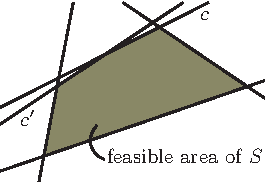
\includegraphics[scale=0.9]{figures/almostRedundant.pdf}
	\caption{The inequality $c$ is almost redundant compared to $c'$, and vice versa.}
	\label{fig:almostRedundant}
\end{figure}

Thus, instead of only collecting a set of redundant inequalities, the manager also collects a set of almost redundant inequalities; the property is checked by the workers simultaneously with the ordinary redundancy check. After the parallel redundancy check, \emph{one} worker then goes through all the almost redundant inequalities one by one and removes the ones that are still almost redundant. The almost redundant inequalities found this way is then removed from the system $S$.  

Almost redundant inequalities can \emph{not} be removed in parallel. Otherwise, in a situation as in Figure~\ref{fig:almostRedundant}, both $c$ and $c'$ could simultaneously be found almost redundant by two different workers, causing them both to be eliminated. When removing almost redundant inequalities sequentially, both inequalities would be checked again, but only the one examined first would be removed.

A method for coarsening the boundary of the feasible area that relies on removing almost redundant inequalities are used in \cite{lukatskii08} and \cite{shapot12} too, though the approach is different.

\subsection*{Preprocessing}
Prior to projecting the system we perform some simple preprocessing steps in order to have a smaller system as the starting point. The steps (which can be found in e.g. \cite{brearley75}, \cite{andersen95} and \cite{maros})
are then applied repeatedly in a cycle, as long as ``something happens'' in a cycle, that is, an (in)equality or variable in $Y$ is removed, a variable is substituted with a value, or a bound of a variable or an (in)equality's left-hand-side is updated.
%When doing this, variables in $\VAR(S)\setminus Y$ are not removed, and we keep track of any values that they are substituted with. 

The individual preprocessing steps are as follows; details can be found in \cite{MyTechRep}.
%
\begin{enumerate} \itemsep0em
	\item Remove all empty inequalities, i.e. inequalities $c$ where $\mi{var}(c)=\emptyset$, and remove all unused variables $x\in Y$.
\setcounter{counterName}{\value{enumi}}
\end{enumerate}
For each variable $x$, we maintain an upper and lower bound, $ub_x$ and $lb_x$, which initially is $\pm$ infinity.
\begin{enumerate} \itemsep0em
\setcounter{enumi}{\value{counterName}}
	\item If $ub_x = lb_x$ for a variable $x\in X$, then substitute $x$ with $lb_x$ in all (in)equalities in $S$. 
	\item If an inequality $a_x\cdot x \leq b$ belongs to $S$, then remove it from $S$. If $a_x>0$ then update the upper bound for $x$ to $\min\{ub_x,\frac{b}{a_x}\}$, otherwise update the lower bound to $\max\{lb_x,\frac{b}{a_x}\}$.
For the equality $a\cdot x = b$, both bounds are updated.
	\item If $\Neg_S(x)=\emptyset$ for an $x\in Y$ (implying that $x$ does not occur in an equality) then remove $\Pos_S(x)$ from $S$. If $\Neg_S(x)$ only consist of the inequality defining the lower bound of $x$ then substitute $x$ with $lb_x$ in all (in)equalities in $S$. Similarly w.r.t. $\Pos_S(x)$. We notice that this is \emph{not} a normal preprocessing step, but corresponds to doing FME on $x$, which changes the feasible area of $S$. 
\setcounter{counterName}{\value{enumi}}
\end{enumerate}
For each inequality we also maintain an upper and lower bound (which potentially is $\pm$ infinity) for its left-hand-side. At a feasible point for $S$, the upper bound for the (in)equality $c$ with left-hand-side $\ve{a}\cdot\ve{x}$ is thus $\mi{high}^c = \smashoperator[r]{\sum_{x. a_x>0}}a_x\cdot ub_x + \smashoperator[r]{\sum_{x.a_x<0}}a_x\cdot lb_x$. Similarly, $c$'s lower bound is given by $\mi{low}^c = \smashoperator[r]{\sum_{x.a_x>0}}a_x\cdot lb_x + \smashoperator[r]{\sum_{x.a_x<0}}a_x\cdot ub_x$.
These bounds might again imply tighter bounds for the variables. 
\begin{enumerate} \itemsep0em
\setcounter{enumi}{\value{counterName}}
	\item If $c$ is an inequality with right-hand-side $b$ and $\mi{high}^c \leq b$ then $c$ is redundant and removed. If instead $c$ is an equality (and still $\mi{high}^c \leq b$) then necessarily $\mi{high}^c = b$, and $c$ is removed from $S$ while all positive (negative) variables in $c$ is replaced with their upper (lower) bound.
	\item If $c$ is an (in)equality with right-hand-side $b$, and $\mi{low}^c \geq b$, then neccessarily $\mi{low}^c = b^c$, and $c$ is removed from $S$ while all positive (negative) variables in $c$ are replaced with their lower (upper) bound.
	\item For any variable $x$ used by $c$, if $a_x > 0$ and $\mi{low}_x^c<+\infty$, 
	where $\mi{low}_x^c = \smashoperator[r]{\sum_{x'.a_{x'}>0, x'\neq x}}a_{x'}\cdot lb_{x'} + \smashoperator[r]{\sum_{x'.a_{x'}<0}}a_{x'}\cdot ub_{x'}$, 
	then $ub_x$ is updated to $\min\{ub_x, \frac{b-\mathit{low}_x^c}{a_x}\}$. 
	Similarly, if $a_x < 0$ and $\mi{low}_x^c<+\infty$, then $lb_x$ is updated to $\max\{lb_x, \frac{b-\mathit{low}_x^c}{a_x}\}$.	
	Updating bounds for (in)equalities with only one variable (step 3) is a special case of this.
\setcounter{counterName}{\value{enumi}}
\end{enumerate}	
%
Comparing two inequalities syntactically, we can in some cases detect redundancy as described below. All pairs of inequalites are then compared in an efficient manner.
In the following, let $c$ be an (in)equality in $S$ with left-hand-side $\ve{a}\cdot \ve{x}$ and right-hand-side $b$, and let $c'$ be another (in)equality with left-hand-side $\ve{a}'\cdot \ve{x}$ and right-hand-side $b'$. 
\begin{enumerate} \itemsep0em
\setcounter{enumi}{\value{counterName}}
\item 
If $\ve{a}=\sigma\cdot \ve{a}'$, then $c$ is \emph{linearly dependent} (\cite{lassez93}). $c$ is hence redundant if
it is an \underline{in}equality, and either $\sigma\geq 0$ and $\sigma\cdot b'\leq b$; or $c'$ is an equality, $\sigma<0$ and $\sigma\cdot b'\leq b$. $c$ is also redundant if both $c$ and $c'$ are equalities and $\sigma\cdot b'\leq b$. 
It is enough to check if this holds for $\sigma = \frac{c_x}{c'_x}$ for the first variable $x$ used by $c'$.
\item
If all variables used in $c$ and $c'$ are non-negative, and there exists a $\sigma\geq 0$ such that $a_i \leq \sigma \cdot a'_i$ for all $i$, while $\sigma\cdot b' \leq b$, then $c$ is \emph{less strict} than $c'$; it is redundant and hence removed. If $c$ is an equality, so must $c'$ be, and hence $c'$ is turned into an equality. 
This is only required to be tested for specific value of $\sigma$ that depends on whether $c'$ has a variable with a negative coefficient or not; see \cite{MyTechRep}.
\end{enumerate} 
%\end{document}